\documentclass[tikz, border=10pt]{standalone}
\usetikzlibrary{positioning, arrows.meta, bending, decorations.text}

\begin{document}
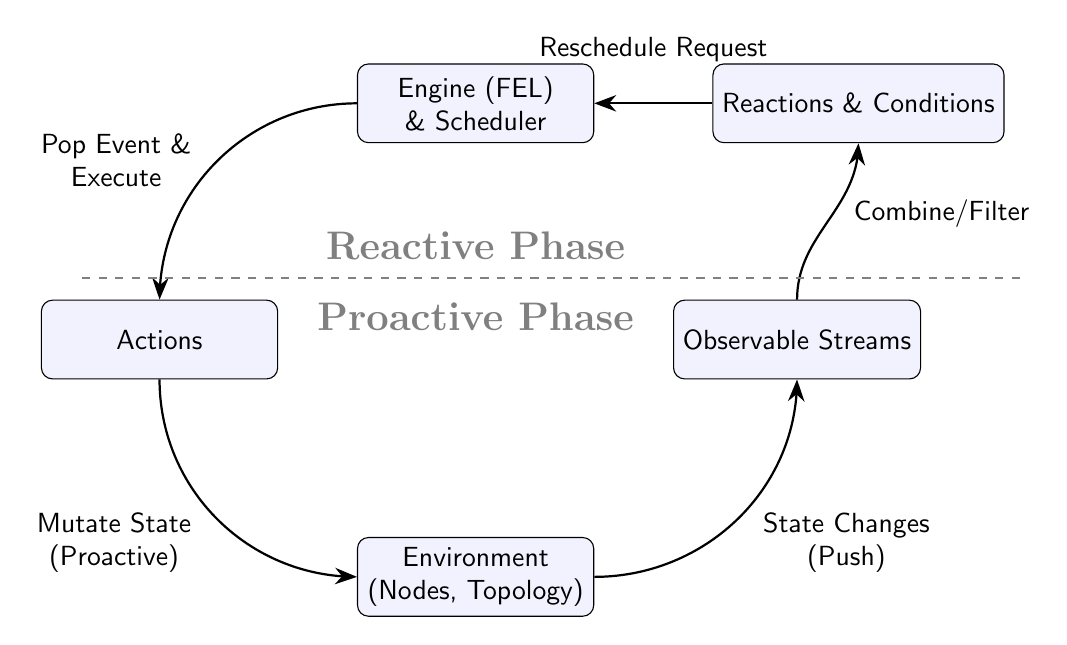
\begin{tikzpicture}[
	box/.style={draw, rectangle, rounded corners, minimum width=3cm, minimum height=1cm, align=center, fill=blue!5},
	arrow/.style={-{Stealth[scale=1.2]}, thick},
	font=\sffamily
	]

	\node[box] (env) {Environment \\ (Nodes, Topology)};
	\node[box, above right=2cm and 1cm of env] (streams) {Observable Streams};
	\node[box, above left=2cm and 1cm of env] (actions) {Actions};
	\node[box, above=5cm of env] (engine) {Engine (FEL) \\ \& Scheduler};
	\node[box, right=1.5cm of engine] (reactions) {Reactions \& Conditions};

	\draw[arrow] (env.east) to[out=0, in=270] node[right, align=center, xshift=0.2cm, yshift=-0.3cm] {State Changes \\ (Push)} (streams.south);
	\draw[arrow] (streams.north) to[out=90, in=270] node[right, xshift=0.2cm, yshift=0.1cm] {Combine/Filter} (reactions.south);
	\draw[arrow] (reactions.west) -- node[above, yshift=0.4cm] {Reschedule Request} (engine.east);

	\draw[arrow] (engine.west) to[out=180, in=90] node[left, align=center, xshift=-0.2cm] {Pop Event \& \\ Execute} (actions.north);
	\draw[arrow] (actions.south) to[out=270, in=180] node[left, align=center, xshift=-0.2cm, yshift=-0.3cm] {Mutate State \\ (Proactive)} (env.west);

	\draw[dashed, gray, thick] (-5, 3.8) -- (7, 3.8);

	\node[font=\bfseries\Large, text=gray, below=1.0cm of engine.south] {Reactive Phase};
	\node[font=\bfseries\Large, text=gray, above=2.5cm of env.north] {Proactive Phase};

\end{tikzpicture}
\end{document}
